\chapter{タスク2：液体を注ぐ作業}
\label{ch:pour}
% ============================================================================

本章では，第\ref{ch:introduction}章で示した形状および環境・道具の分析観点を，
料理作業において高い頻度で現れる「注ぐ」動作に適用する．
注ぎ作業は，直接把持できない液体を対象とし，容器という環境を介して間接的に操作する点に
特徴がある．したがって，本作業は第\ref{ch:introduction}章の表\ref{tab:tasks}に示した
「容器間関係（環境的な分析）」と「容積・形状（幾何学的な分析）」の検証に位置づけられる．

本章では，第\ref{ch:system}章で構築した容器の3D点群モデルを基盤とし，
幾何学的な分析による注いだ体積の推定と，動作制御による精密な注ぎ実行を統合することで，
\revise{事前登録していない形状の容器に対して，容器形状を液体量または目標角度へ変換し，制御中に計量カップや秤を用いない定量注ぎを実現する二つのタスク固有手法を提案する．}

本章の構成は以下の通りである．
まず\ref{sec:pour_problem_overview}節で注ぎ作業の問題設定と提案手法の全体像を述べる．
次に\ref{sec:pour_analysis}節では，本手法のコアとなる幾何学的な分析として，
液面検出による注いだ体積の推定，注ぎ口形状の認識，および注ぎ角度と注いだ量の関係の計算について
述べる．
\ref{sec:pour_control}節では，分析結果に基づく動作制御として，
注いだ液体の量でフィードバックし，注ぐ容器の回転角速度のPD制御と注ぐ容器の回転角度のP制御
の2つの制御手法を述べる．
\ref{sec:pour_experiment}節では，形状特性の異なる複数容器を用いた実験により
提案手法の有効性を検証する．
最後に\ref{sec:pour_summary}節で本章を総括する．


% ============================================================================
\section{問題設定と提案手法の概要}
\label{sec:pour_problem_overview}
% ============================================================================

\begin{revisionblock}
\subsection{想定する状況，目的および適用条件}
本章は，家庭の調理中に，水，牛乳，だし等の低粘性液体を一つの開口容器から別の開口容器へ指定量だけ移す状況を想定する．
ロボットには注ぐ操作，使用する二容器，目標体積 $V_{\mathrm{tar}}$，および把持方法が与えられており，対象容器の形状に応じた液量または傾斜角度が未決定である．
液体・容器の選択，レシピからの目標量抽出，容器の初期配置，こぼれ後の清掃，および複数工程の切替えは対象外とする．

手法1では注ぎ先容器の内面と注ぎ中の液面を観測できること，手法2では注ぐ容器の形状と初期液体体積が得られることを前提とする．
両手法とも，容器を剛体，液体を水・牛乳程度の低粘性流体とし，注ぎ先への流れが遮られない状況を扱う．
本章の達成目標は，容器ごとの事前登録モデルなしに，その場で得た容器形状から液面高さ・体積関係または傾斜角度・流出量関係を求め，設定した条件下で指定量を注ぐことである．
\end{revisionblock}

\subsection{注ぎ作業の定式化と技術的課題}

料理作業において，注ぎ作業は液体調味料（酢，醤油など）の投入や水の添加など，
高い頻度で現れる基本操作である．
レシピに示された分量通りに定量的に注がなければ，料理の味や食感が変わってしまうため，
注ぐ量の定量性は調理の成否に直結する．

人間が定量的な注ぎを行う場合，計量カップ，計量スプーン，あるいは秤を用いて
液体の体積を計量するのが一般的である．
しかし，このような道具を用いる方法では，正確な分量を計量できる反面，
計量作業を別途実施しなければならないという問題がある．
例えば，水を複数のコップに均等に分ける場合，容器ごとに体積を計量する必要があるため，
作業時間が増大する．
\begin{revisionblock}
ロボットが容器形状を直接計測して液体体積を計算できれば，計量専用容器への移替え，追加の把持・搬送，および使用後の洗浄を省き，注ぎ先容器へ直接移すことができる．
また，同一液体を複数容器へ分配する場合には，各容器を秤へ移動することなく連続して作業できる．
一方，計量カップや秤は既に簡便で高精度な手段であり，本研究はそれらが不要であることを主張するものではない．
本手法の利点は，既存の視覚・操作系だけで容器形状を制御量へ変換し，補助器具と作業工程を減らせる点にあり，必要精度，観測可能性，清掃性に応じて従来の計量手段と使い分けるべきである．
\end{revisionblock}

したがって，本研究で解決すべき課題は次のように定式化される：

\begin{quote}
  事前に形状が未知である注ぐ容器から，
  同じく形状が未知である注ぎ先容器へ，
  計量カップや秤などの外部計測道具を用いることなく，
  指定された目標体積 $V_{\mathrm{tar}}$ の液体を精密に注ぐこと．
\end{quote}

この課題を実現するためには，以下の2つの中核的課題を解決する必要がある：

\begin{description}
  \item[課題1] 注いだ体積の測定．
    注いだ体積が不明であれば「定量的」とは言えない．
    したがって，注いだ体積の測定は本研究の中心であり，
    \revise{対象容器ごとの事前モデルに依存せず，その場で計測した形状から体積を求められる方法が必要となる．}
  \item[課題2] 注ぎ動作の制御．
    注いだ体積が推定できたとしても，注ぎ動作の制御が高精度に行えなければ，
    液体がこぼれたり，一気に大量の液体が注いだりする可能性がある．
    これは誤差の原因となるため，注いでいる間における注ぐ容器の傾き角度の制御が重要である．
\end{description}


\subsection{提案手法の概要}

上記の2つの課題に対し，注ぎ作業には注ぐ容器と注ぎ先容器の2つの容器が関連することから，
本研究ではそれぞれの容器に着目した2つの方法論を提案する．

\begin{enumerate}
  \item \textbf{手法1：注ぎ先容器に注目} 
    　注ぎ先容器の3Dモデルと，注いでいる間にリアルタイム検出される液面高さから
    現在注いだ体積を推定する．その体積誤差に基づくPD制御により
    注ぐ容器の傾き角速度を操作する方法である．
    この手法の利点は，注ぐ容器の状態や形状が未知であっても正確に注げる点にあるが，
    注ぎ先容器の内部形状が計測できない場合には適用できない．
  
  \item \textbf{手法2：注ぐ容器に注目} 
    　注ぐ容器の3Dモデルと初期液体の量から注ぎ口形状を認識し，
    容器の傾き角度と注いだ体積の関係を事前に計算する．
    この関係に基づき，目標体積に対応する目標角度まで注ぐ容器を回転させる
    P制御により注ぎを実行する方法である．
    この手法は手法１の欠点（注ぎ先容器の内部計測不能時）を補完できる一方，
    注ぐ容器の形状と初期液体の量が計測できない場合には適用できない．
\end{enumerate}

2つの手法を合わせて使用することで，注ぐ容器か注ぎ先容器のどちらか一方の
3Dモデルが取得可能であれば，注いだ体積の測定と動作制御が可能となる．

両手法に共通する基盤として，第\ref{ch:system}章で述べた手順により
容器の3D点群モデルを事前に取得する．
また，容器モデルからの部分容積計算についても第\ref{ch:system}章の
スライス断面積積分に基づく手法を前提とするが，
本章では特に，任意の液面高さ $H$ および容器姿勢 $\theta$ における
容器下部の体積 $V_{H,\theta}$ を，

\begin{equation}
  V_{H,\theta} = \int_{0}^{H} S(h,\theta)\,dh
  \label{eq:pour_volume_integral}
\end{equation}

と表す．
ここで $S(h,\theta)$ は，容器モデルを高さ $h$ の水平面で切断したときの断面積であり，
容器の傾き角度 $\theta$ に依存する関数である．
式(\ref{eq:pour_volume_integral})の離散化計算は，
モデルを $z$ 軸に沿って高さ $h_\delta$ の $N$ 個の部分に分割し，
各部分の体積 $V_n$ を上下断面積の台形近似により求め，
それらの総和として計算する：

\begin{equation}
  V_n \approx \frac{(S_{n-1} + S_n)\,h_\delta}{2}, \quad
  V_{H,\theta} = \sum_{n=1}^{N} V_n
  \label{eq:pour_volume_discrete}
\end{equation}

ここで $h_\delta = H/N$，$S_n = S(h_\delta \cdot n,\;\theta)$ である．
各断面の面積 $S_n$ は，スライス断面に含まれる点群をスライス平面に投影した後，
ConvexHull を用いて計算する．

% -------------------- IROS2019 Fig. ParametersV4 --------------------
\begin{figure}[t]
	\vspace{3mm}
	\centering
	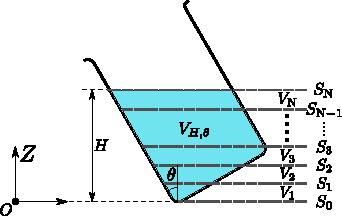
\includegraphics[width=.8\linewidth]{fig/chp_pouring/ParametersV4.pdf}
	\caption{
		$V_H$ is the volume that we want to calculate.
		$H$ is the height, and can be set between the bottom of the model and top of the model.
		To calculate the integration, $S_0, S_1, S_2, \dots, S_N$ are the areas of each cross-sectional plane. $V_1, V_2, V_3, \dots, V_N$ are the volumes of each slice part.}
	\label{fig:pour_ParametersV4}
\end{figure}
% -------------------------------------------------------------------


% ============================================================================
\section{注ぎ作業のための幾何学的な分析}
\label{sec:pour_analysis}
% ============================================================================

本節では，提案手法の幾何学的な分析として，
注ぎ先容器を対象とした液面検出に基づく注いだ体積のリアルタイム推定
（\ref{sec:pour_liquid_level}節），
注ぐ容器を対象とした注ぎ口形状の認識（\ref{sec:pour_edge_point}節），
注ぎ角度と注いだ体積の関係計算（\ref{sec:pour_angle_volume}節）
について述べる．

% ---------------------------------------------------------------------------
\subsection{液面による注いだ体積の推定}
\label{sec:pour_liquid_level}
% ---------------------------------------------------------------------------

手法1では，注いでいる間に注ぎ先容器内の液面をリアルタイムで検出し，
その高さから現在注いだ体積を推定する必要がある．
醤油や酢，油などの料理によく使われる液体は流動性が高く，
大きな外力が加わらない限り液面は常に水平面と平行になる．
この特性を利用し，注ぎ先容器モデルの底面から液面までの間の体積を
注がれた液体の体積とみなす．

\subsubsection{RANSAC による液面検出}

液面検出は，注いでいる間にカメラから取得される各フレームの点群に対して
以下の手順で行う．

\begin{enumerate}
  \item 事前に計算した注ぎ先容器のAABBを用いて，
        PassThroughフィルタにより容器外部の点を除去し，
        容器内部近傍の点群のみを抽出する．
  \item 抽出された点群に対し，RANSACを適用し，
        最も多くのインライアが得られる平面を検出する．
  \item 検出された平面を液面とみなし，その高さ $H_{\mathrm{liquid}}$ を
        容器底面を基準とする座標系での $z$ 座標値として取得する．
\end{enumerate}

RANSAC による平面検出を用いれば，液面以外の構造（容器側壁，底面，ノイズ点）が
混在する点群からでも，液面を安定に抽出できるため，本作業に適している．

\subsubsection{液面高さから注いだ体積への変換}

検出された液面高さ $H_{\mathrm{liquid}}$ を用いて，
現在注いだ体積 $V_{\mathrm{pour}}$ は式(\ref{eq:pour_volume_integral})により
以下のように計算される：

\begin{equation}
  V_{\mathrm{pour}} = V_{H_{\mathrm{liquid}},\,\theta_{\mathrm{target}}}
  = \int_{0}^{H_{\mathrm{liquid}}} S(h,\theta_{\mathrm{target}})\,dh
\end{equation}

ここで $\theta_{\mathrm{target}}$ は注ぎ先容器の傾き角度であり，
注いでいる間は一定と仮定する．
これにより，各制御ステップにおいて現在注いだ体積 $V_{\mathrm{now}}$ が得られ，
目標体積 $V_{\mathrm{tar}}$ との誤差

\begin{equation}
  V_{\mathrm{error}} = V_{\mathrm{tar}} - V_{\mathrm{now}}
  \label{eq:pour_verror}
\end{equation}

がPD制御への入力として用いられる．

% ---------------------------------------------------------------------------
\subsection{注ぐ容器の注ぎ口形状の認識}
\label{sec:pour_edge_point}
% ---------------------------------------------------------------------------

手法2では，注ぐ容器を傾けた際に液体が流出する「注ぎ口」の幾何学的特徴を
事前に求める必要がある．
注ぎ口の認識は，(a) 注ぎ縁の検出と，(b) 注ぐポイントの検出，
の2段階で構成される．

\subsubsection{注ぎ縁の検出}

注ぎ縁とは，容器内部から外部へと通じる開口部の縁である．
容器をスライスしたとき，注ぎ縁を含む断面には必ず不連続な部分が生じる．
この不連続部分の端点を集めることで，注ぎ縁を検出できる．

具体的な検出手順を以下に示す．

\begin{enumerate}
  \item 容器モデルに対し，複数の変換行列 $\mathbf{T}_k\;(k=1,\dots,K)$ を適用し，
        異なる姿勢での点群を生成する．
  \item 各姿勢において，モデルを $z$ 軸方向に1\,mm間隔でスライスし，
        各スライス断面の点群を取得する．
  \item 各断面点群に対し，PCL の ConvexHull モジュールを用いて凸包を計算する．
        ConvexHull の結果は順序付けられた配列で得られるため，
        断面形状に沿った隣接点関係が定まる．
  \item ConvexHull 上の隣接する2点に対し，
        その2点を結ぶ直線から半径 $r = 2.5\,\mathrm{mm}$ 以内にある
        内部点を抽出し，直線上に投影する．
  \item 投影点間の距離を計算し，距離が閾値 $D_T = 2.5\,\mathrm{mm}$ より
        大きい点対を不連続部分の端点として検出する．
  \item 検出された端点群を逆変換 $\mathbf{T}_k^{-1}$ により
        元のモデル座標系へ戻し，全姿勢の結果を統合して注ぎ縁点群を得る．
\end{enumerate}

% -------------------- IROS2019 Fig. pour-edge-1 and pour-edge-2 --------------------
\begin{figure}[t]
	\vspace{3mm}
	\centering
	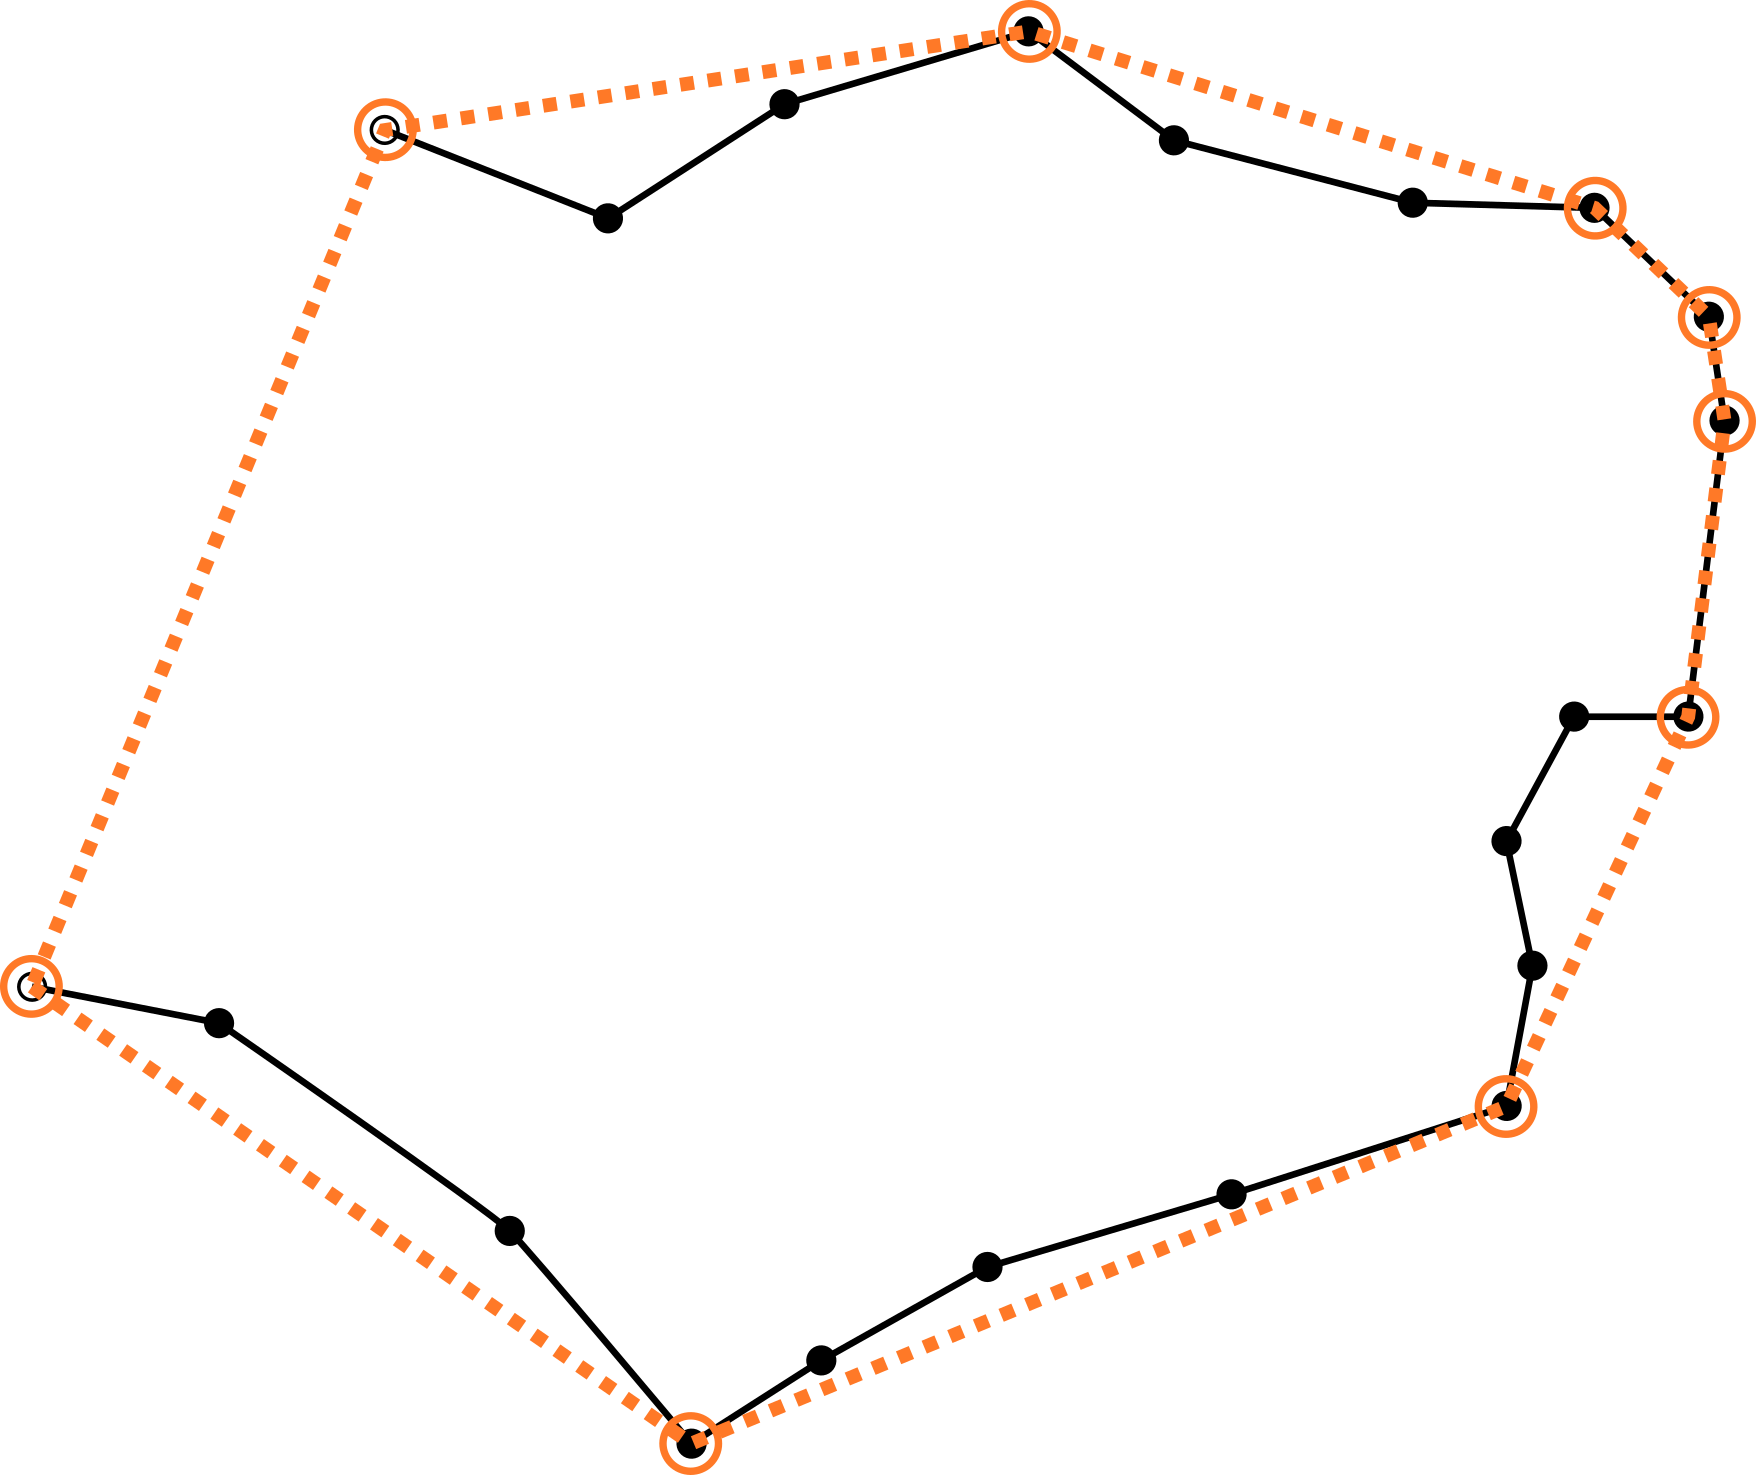
\includegraphics[width=0.57\linewidth]{fig/chp_pouring/PourEdgeConvexHull.png}
	\caption{
		Black points are the cross-sectional point set.
		Black circles mark the endpoints that need to be found.
		Points surrounded by orange circles are the results of \cite{PCL-Convex}, and these points are stored in an ordered array (marked with an orange broken line).
	}
	\label{fig:pour_pour-edge-1}
\end{figure}

\begin{figure}[t]
	\vspace{3mm}
	\centering
	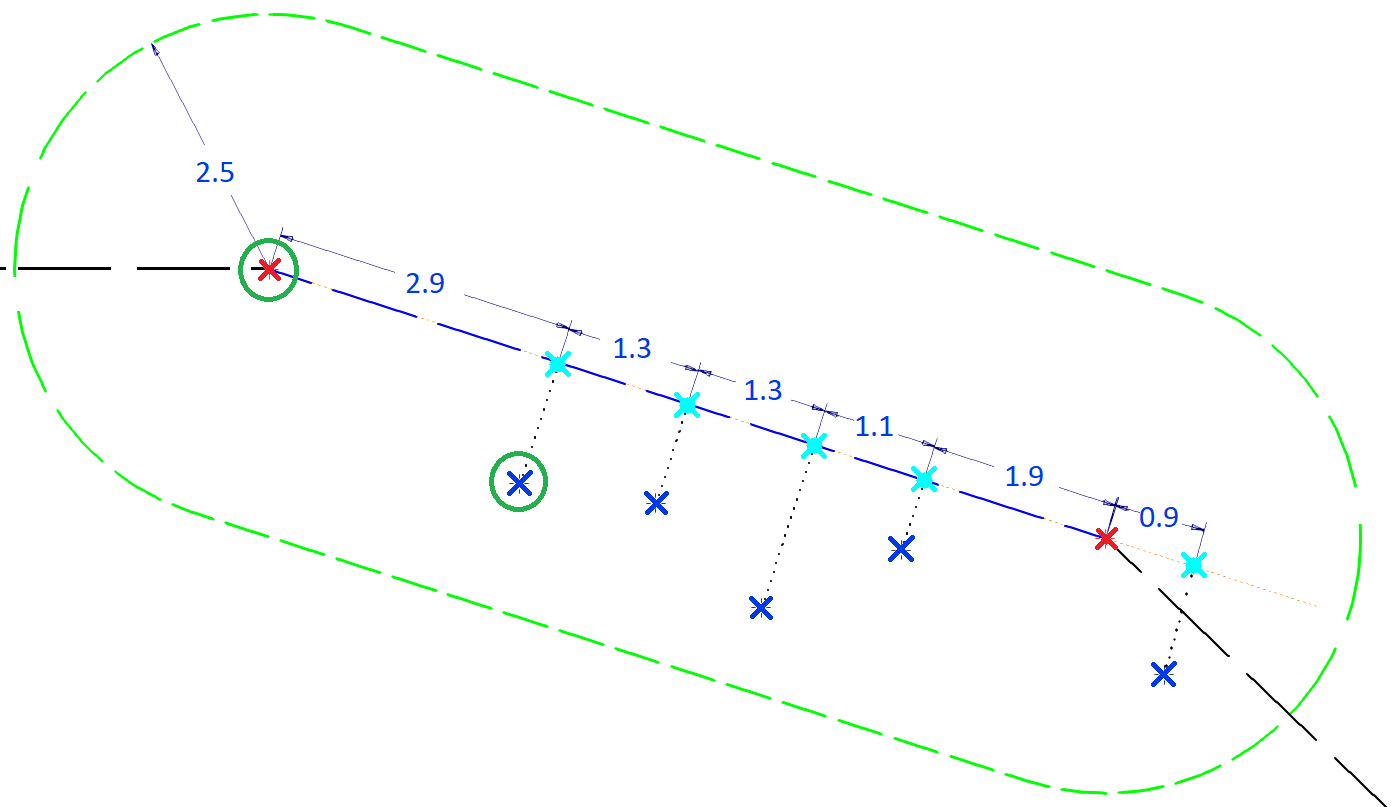
\includegraphics[width=0.9\linewidth]{fig/chp_pouring/pour-edge-2.png}
	\caption{
		This figure shows the point and its neighbor on the convex hull.
		Blue and black broken lines and red crosses are the results of the convex hull. Black broken lines are not related to the endpoints analysis.
		The green broken line is the border of points that will be analyzed.
		Deep blue crosses mark the inner points of the cross-sectional shape.
		Cyan crosses mark the inner points that will be projected onto the line defined by the two red crosses.
		Two points surrounded by deep green circles are the resulting endpoints.}
	\label{fig:pour_pour-edge-2}
\end{figure}
% --------------------------------------------------------------------------------

検出された注ぎ縁にはノイズが含まれるため，
PCLのEuclideanClusterExtractionを用いてクラスタリングし，
平均高さと点数が最大のクラスタを最終的な注ぎ縁として採用する．

\subsubsection{注ぐポイントの検出}

注ぎ縁が得られた後，実際に液体が流出する「注ぐポイント」$\mathbf{P}_{\mathrm{pour}}$
を検出する．
凸形状容器において，注ぐポイントは注ぎ縁の最下点として定義される．

検出手順は以下の通りである：

\begin{enumerate}
  \item 注ぎ縁点群を $x$ 軸回りに複数の傾き角度に回転変換し，
        各姿勢における最下点（$z$ 座標が最小の点）を抽出する．
  \item 全姿勢から得られた最下点群を変換行列により統合する．
  \item 統合された点群に Euclidean クラスタリングを適用し，
        平均高さが最も低いクラスタの重心をもって
        注ぐポイント $\mathbf{P}_{\mathrm{pour}}$ とする．
\end{enumerate}

このように，複数姿勢からの投票に基づく手法により，
単一視点では判断が難しい注ぎ口の最下点を安定して検出できる．

% ---------------------------------------------------------------------------
\subsection{注ぎ角度と注いだ体積の関係計算}
\label{sec:pour_angle_volume}
% ---------------------------------------------------------------------------

注ぐポイント $\mathbf{P}_{\mathrm{pour}}$ が検出されると，
注ぐ容器の傾き角度 $\theta$ と注いだ体積 $V_{\mathrm{pour}}$ の関係を計算できる．
本計算では以下の仮定をおく：

\begin{enumerate}
  \item 注ぎの過程で液こぼれはなし（注いだ液体はすべて注ぎ先容器に注いだ）．
  \item 注ぐ容器内の初期液体体積 $V_{\mathrm{init}}$ は既知である．
  \item $V_{\mathrm{init}} > V_{\mathrm{tar}}$，すなわち初期液体体積は目標体積より十分に大きい．
  \item 液体の粘性は低く（水，ミルク程度），液体は容器の形状に沿って変形する．
  \item 表面張力の影響はここでは無視できるものとする．
\end{enumerate}

% -------------------- IROS2019 Fig. Pouring --------------------
\begin{figure}[t]
	\vspace{3mm}
	\centering
	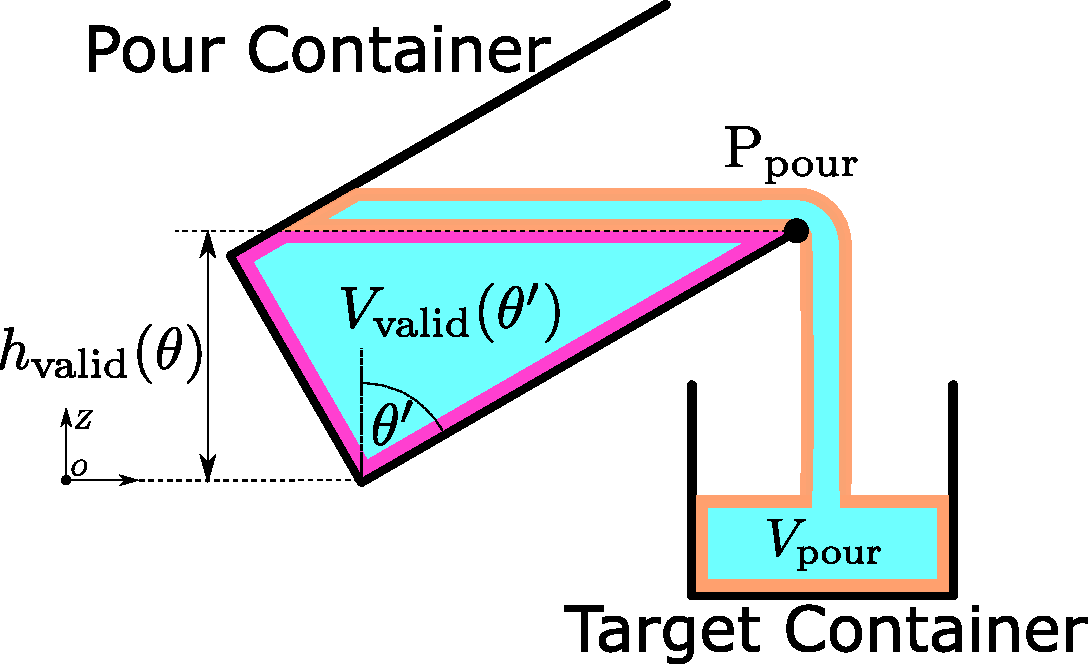
\includegraphics[width=0.7\linewidth]{fig/chp_pouring/Pouring.pdf}
	\caption{
		This figure depicts the pouring scenario when the angle of the pouring container $\theta$ is $\theta^\prime$.
		$\theta^\prime$ is the angle at which the liquid pours out from the pouring container, so $V_\mathrm{valid}(\theta^{\prime})$ (purple frame) is the volume that rests in the pouring container.
		$h_\mathrm{valid}(\theta)$ is defined as the height between the pouring point $\mathrm{P}_\mathrm{pour}$ and the bottom of pouring container.
		$V_\mathrm{pour}$ is the poured volume.
	}
	\label{fig:pour_Pouring}
\end{figure}
% ------------------------------------------------------------

注ぐポイント $\mathbf{P}_{\mathrm{pour}}$ から容器モデル最下点までの
$z$ 軸方向距離を $h_{\mathrm{valid}}(\theta)$ と定義する．
これは傾き角度 $\theta$ の関数であり，$\theta$ における注ぎ口の有効高さを表す．

注ぎ開始前（$\theta = 0^\circ$）の時点では，
$V_{\mathrm{valid}}(0^\circ)$ は容器の最大容積を表し，
$V_{\mathrm{init}}$ はこの容器内に実際に存在する液体の体積である．

注いでいる間の任意の傾き角度 $\theta$ において，
容器内に残された液体の体積 $V_{\mathrm{rest}}$ は常に
$V_{\mathrm{valid}}(\theta)$ と一致する．
すなわち：
\begin{equation}
  V_{\mathrm{valid}}(\theta) = \int_{0}^{h_{\mathrm{valid}}(\theta)} S(h,\theta)\,dh
  = V_{\mathrm{rest}}
\end{equation}

また，注いでいる間，注ぐ容器の液面高さと注ぐポイントの高さは等しく，
かつ注ぐ容器から流出した体積はすべて注ぎ先容器に注がれた体積に等しいという
2つの条件から，
$V_{\mathrm{init}}$，$V_{\mathrm{rest}}$，$V_{\mathrm{pour}}$ の関係は：

\begin{equation}
  V_{\mathrm{init}} = V_{\mathrm{rest}} + V_{\mathrm{pour}}
  = V_{\mathrm{valid}}(\theta) + V_{\mathrm{pour}}
  \label{eq:pour_volume_relation}
\end{equation}

と表される．

したがって，傾き角度 $\theta$ における注いだ体積 $V_{\mathrm{pour}}(\theta)$ は，
以下の式で与えられる：

\begin{equation}
  V_{\mathrm{pour}}(\theta) = 
  \begin{cases}
    0 & \bigl(V_{\mathrm{valid}}(\theta) > V_{\mathrm{init}}\bigr) \\[6pt]
    V_{\mathrm{init}} - V_{\mathrm{valid}}(\theta) & \text{その他}
  \end{cases}
  \quad (0^\circ \leq \theta \leq 180^\circ)
  \label{eq:pour_angle_volume_relation}
\end{equation}

一つ目の場合は，液面がまだ注ぐポイントに到達しておらず，
液体が流出していない状態に対応する．

% ---------------------------------------------------------------------------
\subsection{リアルタイム処理のための変換テーブル}
\label{sec:pour_transform_table}
% ---------------------------------------------------------------------------

\subsubsection{液面高さ→注いだ体積変換テーブル}

手法1の実行時，断面積積分をリアルタイムで毎回計算することは計算負荷が高い．
そこで，容器モデル取得時に，液面高さ $h$ から注いだ体積 $V$ への
変換テーブル $T(h)$ を事前に作成しておく．

具体的には，容器底面 $z_{\mathrm{min}}$ から上面 $z_{\mathrm{max}}$ まで
1\,mm 刻みで各高さ $h_i$ に対応する体積 $V_{h_i}$ を
式(\ref{eq:pour_volume_discrete})により計算し，テーブルとして格納する．
注いでいる間に液面高さ $h$ が検出された際には，テーブル参照と線形補間により
注いだ体積を得る：

\begin{equation}
  V_{\mathrm{output}} = T(\lfloor h \rfloor) 
  + \bigl(T(\lceil h \rceil) - T(\lfloor h \rfloor)\bigr)
  \cdot \bigl(h - \lfloor h \rfloor\bigr)
  \label{eq:pour_table_interp}
\end{equation}

これにより，注いでいる間の計算コストを大幅に低減し，
高い制御周期を維持することが可能となる．

\subsubsection{傾き角度→注いだ体積変換テーブルのノイズ処理}

手法2についても，\ref{sec:pour_angle_volume}節の方法で
傾き角度 $\theta$ から注いだ体積 $V_{\mathrm{pour}}$ への変換テーブルを作成する．
しかし，点群モデルのノイズの影響により，角度の増加に伴って
計算上の注いだ体積が一時的に減少する現象が生じる場合がある．
これは，実際には角度増加時に注いだ体積が減少することはありえないため，
誤差の原因となる．

この問題に対し，変換テーブルにおいて注いだ体積の減少が検出された区間では，
線形補間を用いてデータを補正する．
具体的には，減少開始点と減少終了点の間を直線で補間することで，
単調増加性を保証したテーブルを得る．

さらに，注ぎ実行時には目標体積から目標角度を逆引きする必要があるため，
注いだ体積から傾き角度への逆変換テーブルをバイナリサーチにより作成する．
これにより，目標体積 $V_{\mathrm{tar}}$ に対応する目標角度 $\theta_{\mathrm{tar}}$ が
$O(\log N)$ で探索可能となる．


% ============================================================================
\section{動作制御}
\label{sec:pour_control}
% ============================================================================

前節の幾何学的な分析により得られた注いだ体積の推定に基づき，
本節では2つの手法のための実際にロボットの注ぎ動作の制御について述べる．
いずれの手法においても，注ぎ動作は「傾き制御」と注ぎ停止後の「戻し動作」の
2つの段階で構成される．

% ---------------------------------------------------------------------------
\subsection{手法1の制御：注いだ体積積をフィードバックするPD制御}
\label{sec:pour_method1_pd_control}
% ---------------------------------------------------------------------------

手法1では，\ref{sec:pour_liquid_level}節で述べた液面検出により
リアルタイムに推定される注いだ体積をフィードバックとして，
注ぐ容器の傾き角速度 $\omega$ をPD制御により操作する．

\subsubsection{PD制御則の設計}

注ぎ作業において，一度注がれた液体は注ぐ容器に戻らないという特性がある．
このため，体積誤差 $V_{\mathrm{error}}$（式(\ref{eq:pour_verror})）の積分項は
常に増大し続け，目標値に達しても注ぎを継続する方向に作用してしまう．
したがって，I制御を含むPID制御は本作業に不向きであり，
積分項を省略したPD制御を採用する．

制御則は以下の通りである：

\begin{equation}
  \omega = k_p\,V_{\mathrm{error}} + k_d\,D_{\mathrm{error}}
  \label{eq:pour_pd_control}
\end{equation}

ここで $k_p$ は比例ゲイン，$k_d$ は微分ゲインであり，
$D_{\mathrm{error}}$ は注いだ体積の増加速度（体積誤差の時間微分）である．

また，$V_{\mathrm{error}}$ が大きい初期段階において，
式(\ref{eq:pour_pd_control})の $\omega$ をそのまま適用すると
一気に大量の液体が注がれてしまう可能性がある．
これを防止するため，角速度 $\omega$ に上下限制約を設ける．
本研究では $-2^\circ/\mathrm{s} \leq \omega \leq 2^\circ/\mathrm{s}$ と設定した．

\subsubsection{停止条件と戻し動作}

注ぎ動作の停止条件は，体積誤差がゼロ以下になった時点とする：

\begin{equation}
  V_{\mathrm{error}} \leq 0
  \label{eq:pour_stop_condition}
\end{equation}

停止条件が満たされた後，液体の増加を可能な限り速やかに停止させるため，
直ちに戻し動作を実行する．
戻し動作では，PDコントローラを停止し，手先座標系を $\omega$ の負の方向に回転させ，
注ぐ容器がテーブルに対して垂直になるまで戻す．
これにより，注ぎ口からの液体の流出を速やかに止め，
目標体積を超える量が注がれるのを防ぐ．

% ---------------------------------------------------------------------------
\subsection{手法2の制御：目標角度をフィードバックするP制御}
\label{sec:pour_method2_p_control}
% ---------------------------------------------------------------------------

手法2では，\ref{sec:pour_angle_volume}節で計算した「角度→注いだ体積」関係に基づき，
目標体積 $V_{\mathrm{tar}}$ に対応する目標角度 $\theta_{\mathrm{tar}}$ を
事前に計算し，この目標角度へのP制御により注ぎを実行する．

\subsubsection{P制御則の設計}

手法2の制御は，手法1よりも単純なP制御で実現される．
目標角度 $\theta_{\mathrm{tar}}$ と現在の傾き角度 $\theta$ の誤差

\begin{equation}
  \theta_{\mathrm{error}} = \theta_{\mathrm{tar}} - \theta
  \label{eq:pour_theta_error}
\end{equation}

に基づき，傾き角速度 $\omega$ を以下のP制御則により決定する：

\begin{equation}
  \omega = k_p\,\theta_{\mathrm{error}}
  \label{eq:pour_p_control}
\end{equation}

手法1と同様に，$\omega$ には上下限制約を設け，
過剰な角速度による液こぼれを防止する．

\subsubsection{停止条件と戻し動作}

制御の停止条件は，角度誤差がゼロ以下となった時点とする：

\begin{equation}
  \theta_{\mathrm{error}} \leq 0
  \label{eq:pour_theta_stop}
\end{equation}

制御停止条件が到達した後，注ぐポイントより高い残留液体が完全に流出するまで
注ぐ容器を現在の傾き角度に $t$ 秒間保持する．
この待機時間は液体の粘性と容器の材質に依存するが，本研究では経験的に設定した．
待機終了後，\ref{sec:pour_method1_pd_control}節と同様の戻し動作を実行し，
注ぎを完了する．


% ============================================================================
\section{実験による検証}
\label{sec:pour_experiment}
% ============================================================================

提案手法の有効性を検証するため，双腕ロボットシステムを用いて
以下に示す実験を実施した．
まず，提案手法の基盤となる容積計算の精度を評価し（\ref{sec:pour_exp_volume_cal}節），
続いて手法1（\ref{sec:pour_exp_method1}節）および
手法2（\ref{sec:pour_exp_method2}節）の注ぎ精度を検証した．
手法2については，表面張力が注ぎ精度に与える影響を別途評価した上で，
総合的な注ぎ精度を評価した．
最後に両手法の比較考察を行う（\ref{sec:pour_exp_discussion}節）．

% ---------------------------------------------------------------------------
\subsection{実験環境と評価指標}
\label{sec:pour_exp_setup}
% ---------------------------------------------------------------------------

\subsubsection{容器}

実験には，形状特性の異なる3種類の容器（図\ref{fig:pour_cups}）を用いた．

\begin{figure}[t]
	\vspace{3mm}
	\centering
	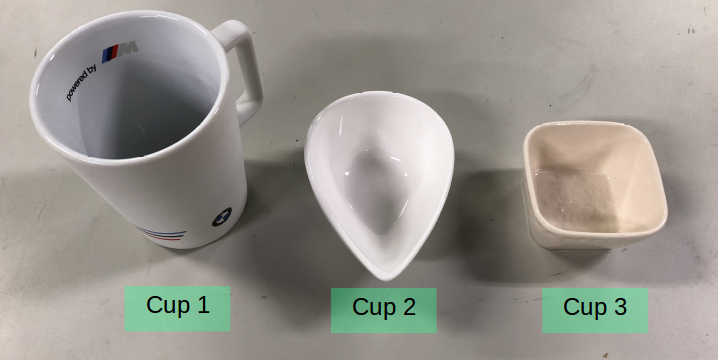
\includegraphics[width=0.8\linewidth]{fig/chp_pouring/Cups-v2.png}
	\caption{Containers used in experiment. Left container is Cup~1, middle is Cup~2, right is Cup~3.  
    % In the experience at Section~\ref{sec:exp0}, each cups had poured 20 times. In the experience of Method~1, each cups had poured 10 times. In the experience of Method~2, Cup~1 was not used, Cup~2 and Cup~3 were poured 15 times each in Section~\ref{sec:method-2-influence-of-surface-tension-on-method-2}, and 10 times each in Section~\ref{sec:Method2-expAll}.
    % TODO: Add right section ref
    }
	\label{fig:pour_cups}
\end{figure}

\begin{enumerate}
  \item \textbf{容器1：} 深さがあり底部が窄まった形状（最大容積 290\,ml）．
  \item \textbf{容器2：} 浅く広口の曲面形状（最大容積 120\,ml）．
  \item \textbf{容器3：} 角が丸い四角形の容器（最大容積 88\,ml）．
\end{enumerate}

手法1の実験では，注ぐ容器は内容量 1000\,ml の牛乳パックを，
注ぎ先容器は容器1--3のすべてをそれぞれ使用した．
手法2の実験では，注ぐ容器は容器1は平行グリッパでの安定把持が困難であったため
容器2および容器3のみを，注ぎ先容器には皿を使用した．


\subsubsection{液体および真値の取得}

実験で使用した液体は以下の通りである．
容積計算精度実験および手法1の実験ではミルクティー（液面検出しやすいため）を使用し，
あらかじめ実測した密度 $\rho = 1.0276\,\mathrm{g/cm^3}$ 
を用いて重量から体積に換算した．
手法2の実験では水道水（$\rho = 1.000\,\mathrm{g/cm^3}$）を使用した．

重量の計測には TANITA KD-320（3\,kg ロードセル）を用い，
測定範囲 0--300\,g では 0.1\,g，300--1500\,g では 0.5\,g の精度で
計測した．

評価指標としては，各試行における目標体積との誤差（注いだ体積 $-$ 目標体積）の
平均と標準偏差を用いる．

% ---------------------------------------------------------------------------
\subsection{容積計算精度の基礎評価}
\label{sec:pour_exp_volume_cal}
% ---------------------------------------------------------------------------

\subsubsection{実験方法}

提案手法の基礎となる容積計算の精度を評価するため，
各容器に対し，計量済みの液体を段階的に追加しながら，
液面検出に基づく容積計算を実施した．
容器1では 50\,ml 刻みで 50--250\,ml の5段階，5試行を実施した．
容器2では 25\,ml 刻み（25--100\,ml），容器3では 15\,ml 刻み（15--60\,ml）
の各4段階，各5試行の追加実験を実施した．
各試行で容器モデルを新規に構築し，液面検出を行った．

\subsubsection{実験結果}

% -------------------- IROS2019 Fig. result-VolumeCal --------------------
\begin{figure}[t]
	\centering
	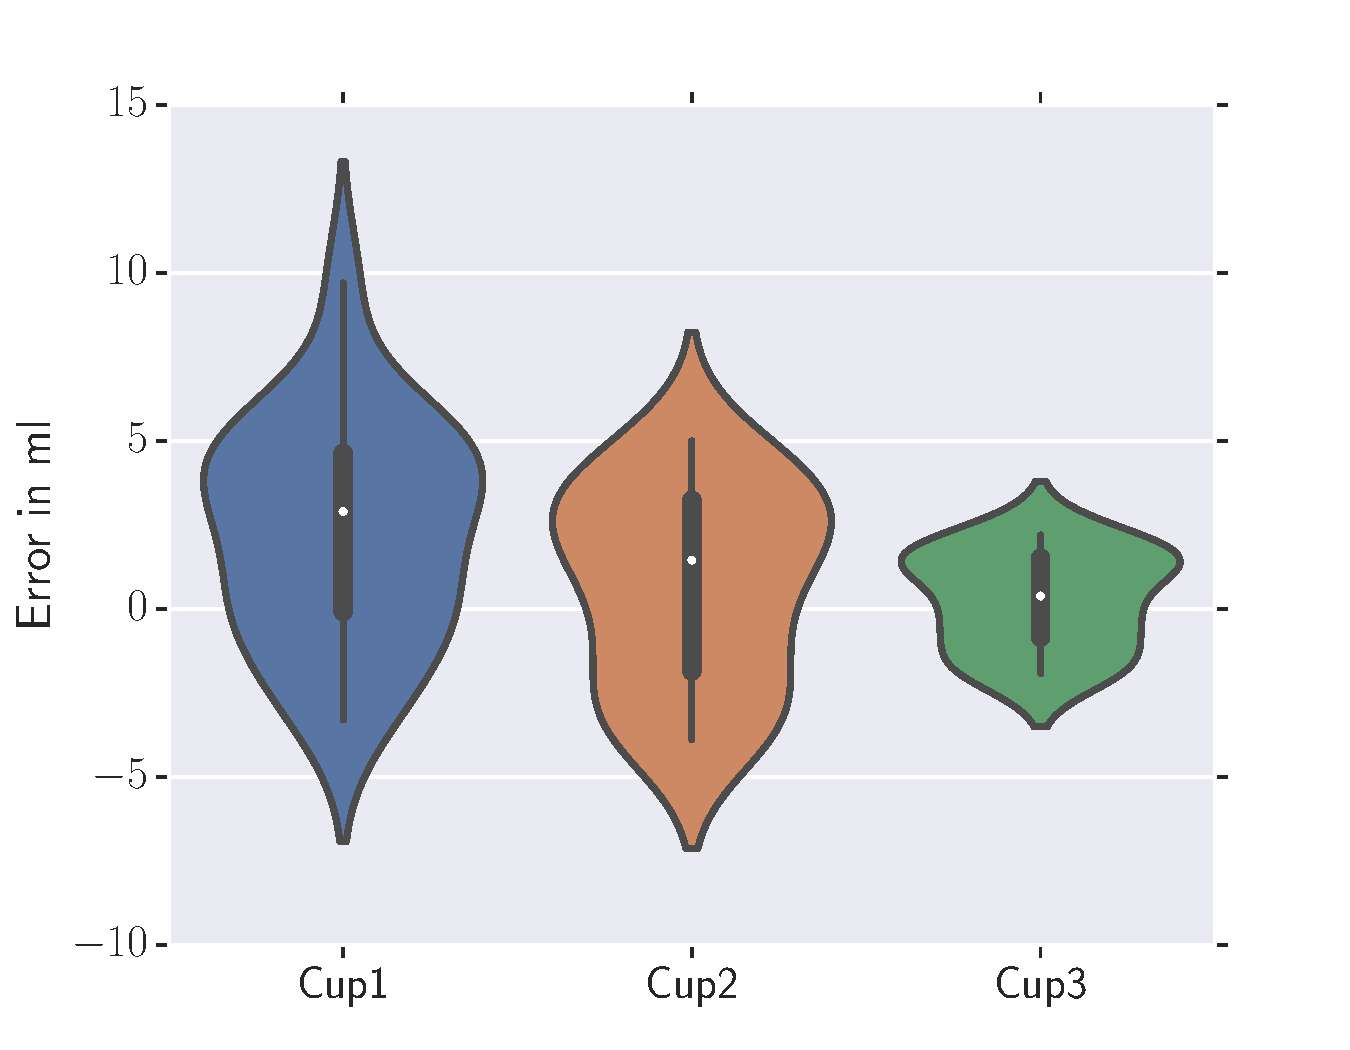
\includegraphics[width=0.8\linewidth]{fig/chp_pouring/VolumeCal.pdf}
	\caption{Results of volume-calculation accuracy. The horizontal axis is type of cup and it also represents the error distribution of each cup. The white dot is the median of errors. The thin black line is the 95\% confidence interval and the thick line is the interquartile range. }
	\label{fig:pour_result-VolumeCal}
\end{figure}
% ------------------------------------------------------------------------

\begin{table}[h]
	\vspace{3mm}
	\caption{The average (Avg.) and standard deviation (S.d.) of errors in volume calculation}
	\label{tab:pour_volume-calculation}
	\centering
	\begin{tabular}{cccc}
		\toprule
		& Cup 1 & Cup 2 & Cup 3 
		\\ \midrule
		Avg. (ml)            & 2.28  & 0.66  & 0.26  
		\\
		S.d. (ml) 			 & 3.29  & 2.94  & 1.44  
		\\ \bottomrule
	\end{tabular}
\end{table}

\subsubsection{考察}
本実験により，提案する体積計算手法の精度が容器形状に依存することが明らかとなった．
容器1では平均誤差2.28\,ml，標準偏差3.29\,mlと3種類中最大の誤差が生じたが，
これは底面が深く窄まった形状のためにカメラで底部まで十分な点群を取得できず，
モデル底面が不完全になることに起因する．
容器2では平均誤差0.66\,ml，標準偏差2.94\,mlであり，
浅く広口の曲面形状によって液面検出時のエッジに歪みが生じ，
RANSACで検出される液面高さが真値より過大評価される傾向が見られた．
一方，角が丸い四角形の容器3は点群取得・液面検出の双方で最も安定した結果を示し，
平均誤差0.26\,ml，標準偏差1.44\,mlという高い精度が得られた．
これらの3Dモデル誤差は，後述の注ぎ精度実験の結果を解釈するに使用する．

% ---------------------------------------------------------------------------
\subsection{手法1の注ぎ精度検証}
\label{sec:pour_exp_method1}
% ---------------------------------------------------------------------------

\subsubsection{実験方法}

手法1の注ぎ精度を評価するため，3種類の注ぎ先容器に対し
それぞれ2段階の目標体積を設定した（容器1：100, 200\,ml；
容器2：45, 90\,ml；容器3：30, 60\,ml）．
各条件で5回の注ぎを実施し，毎回注ぎ先容器のモデルを新規に構築した．

実験手順は以下の通りである：
\begin{enumerate}
  \item テーブル全体を撮影し，容器位置を認識する．
  \item 注ぎ先容器の内部点群を多視点から取得し，3Dモデルを構築する．
  \item 液面高さ--注いだ体積変換テーブルを作成し，容器のAABBを計算する．
  \item 左アームを，注ぎ動作に干渉せず容器内部を観測可能な位置に移動させる．
  \item 右アームで牛乳パックを把持し，注ぎ位置へ移動後，
        左アームのカメラで液面をリアルタイム検出しながら
        PD制御により注ぎを実行する．
  \item 停止条件到達後，戻し動作を実行する．
\end{enumerate}

\subsubsection{実験結果}

% -------------------- IROS2019 Fig. result-Method1 --------------------

\begin{figure}[t]
	\vspace{3mm}
	\centering
	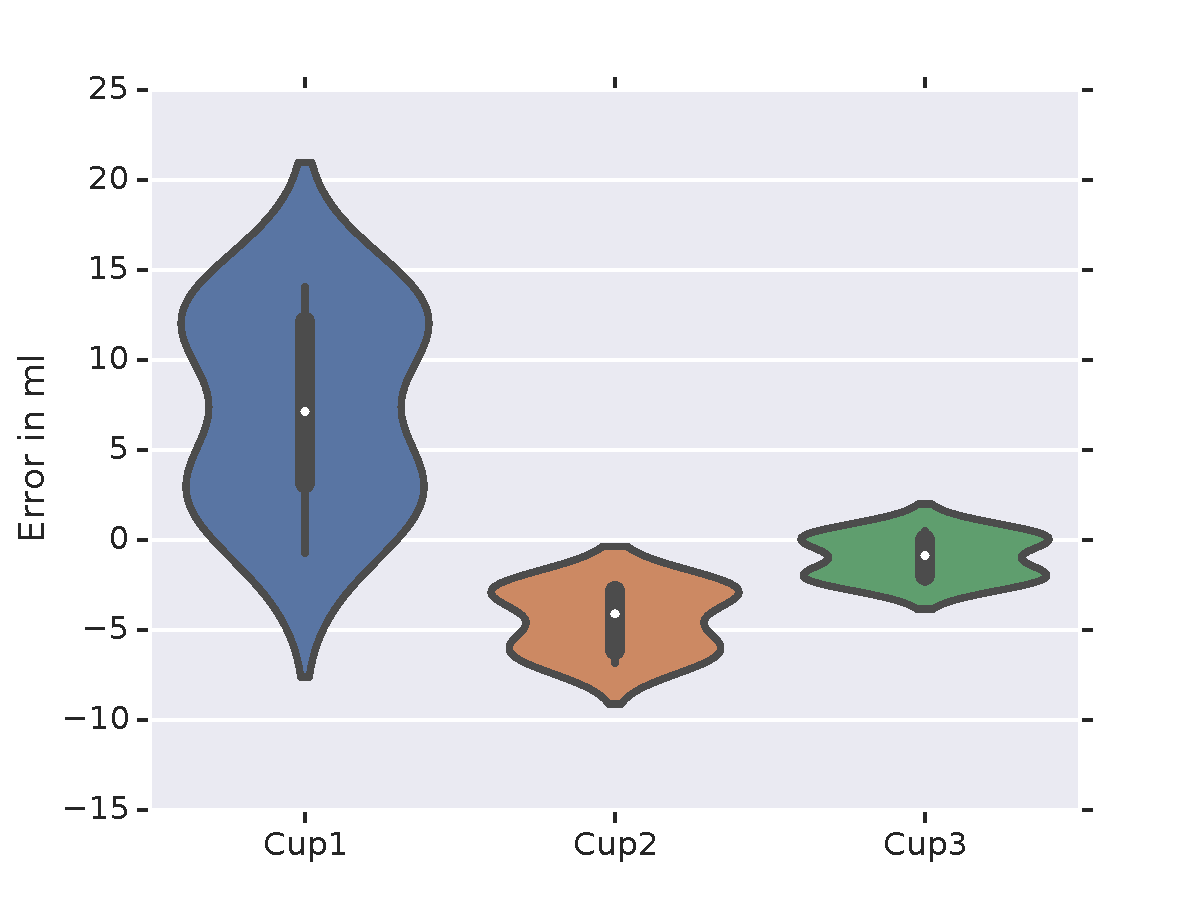
\includegraphics[width=0.8\linewidth]{fig/chp_pouring/Method1-Error.pdf}
	\caption{The accuracy of Method 1}
	\label{fig:pour_result-Method1}
\end{figure}
% ---------------------------------------------------------------------

\begin{table}[htbp]
  \centering
    \caption{The average (Avg.) and standard deviation (S.d.) of errors in  Method~1}
  \label{tab:pour_method1_error}
    \centering
    \begin{tabular}{cccc}
        \toprule
        & Cup 1 & Cup 2 & Cup 3 \\ \midrule
        Avg. (ml)            & 7.35  & -4.43  & -0.95  \\ 
        S.d. (ml) 			 & 5.45  & 1.79  & 1.16 
        \\ \bottomrule
    \end{tabular}
\end{table}

\subsubsection{考察}

手法1の注ぎ精度は容器形状によって大きく異なる結果となった．
容器1では平均誤差7.35\,ml，標準偏差5.45\,mlであり，
これは容積計算実験で確認された底部モデルの不完全性が直接的に影響したものである．
なお本実験では2種類の目標体積のみを設定したため，
図\ref{fig:pour_result-Method1}には二つのピークが現れており，
各ピークが各目標体積における注ぎ誤差の分布を表している．
容器2では平均誤差-4.43\,ml，標準偏差1.79\,mlと負の誤差が生じ，
注いだ液量が容器の容積に近づくにつれて液面と容器の縁が連結し，
液面エッジに歪みが生じて液面高さが高く評価され，
注ぎが早期に停止する現象が確認された．
\revise{容器3では平均誤差$-0.95$\,ml，標準偏差1.16\,mlと本実験中で最も小さい誤差を得た．ただし，この結果は内面と液面を安定に観測できる容器3と，本実験の低粘性・不透明液体に対するものであり，家庭調理全般に十分な性能を示すものではない．}
まとめると，手法1の誤差は容積計算精度実験と同程度の水準に収まっており，
システム全体の誤差は主として体積測定およびモデル精度に起因することが示唆される．


% ---------------------------------------------------------------------------
\subsection{手法2の注ぎ精度検証}
\label{sec:pour_exp_method2}
% ---------------------------------------------------------------------------

手法2では，まず表面張力が角度--注いだ体積関係の推測精度に及ぼす影響を評価し，
その評価を踏まえた上で手法2の注ぎ精度を検証した．

\subsubsection{表面張力の影響評価}
\label{sec:pour_exp_method2_st}

本実験では，\ref{sec:pour_angle_volume}節で提案した角度--注いだ体積関係の
推測アルゴリズムの精度を評価するとともに，表面張力が推測結果に与える
影響を調べた．

\textbf{実験方法：}
容器2および容器3を注ぐ容器とし，各々に初期液体体積を設定した．
容器2では 30, 60, 90\,ml，容器3では 22, 44, 66\,ml の3水準とした．
各初期液体体積に対し，容器を $0^\circ$ から注ぎ終わるまで $5^\circ$ 刻みで
$x$ 軸回りに回転させ，各角度における注いだ体積を秤で計測した．
各条件に対し5回の試行を実施し，毎回容器モデルを新規に取得した．
さらに，表面張力の影響を低減するため，容器の縁に洗剤を薄く塗布した条件
（表面張力なし条件）でも同様の計測を実施した．

\textbf{実験結果：}

% -------------------- IROS2019 Fig. method-exp1 (ST Cup2 and Cup3) --------------------
\begin{figure*}[t]
	\vspace{3mm}
	\centering
	\begin{subfigure}[t]{.45\textwidth}
		\centering
		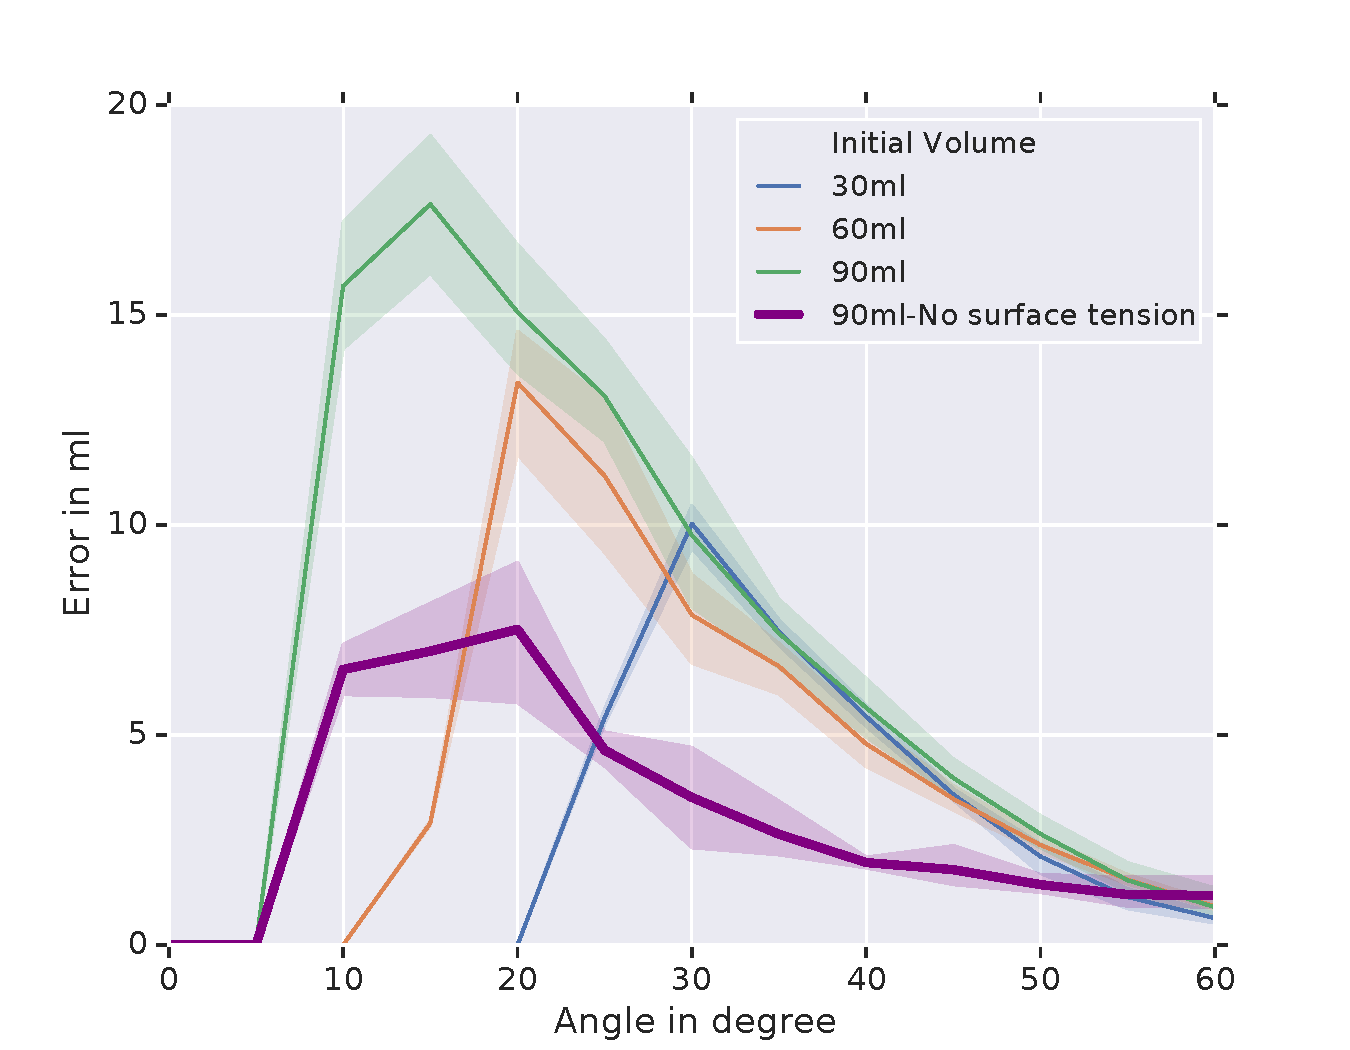
\includegraphics[width=1\textwidth]{fig/chp_pouring/Method2-ST-Cup2-Error.pdf}
		\caption{Errors with Cup~2.}
		\label{fig:pour_method-exp1.sub1}
	\end{subfigure}
	\hspace{1cm}
	\begin{subfigure}[t]{.45\textwidth}
		\centering
		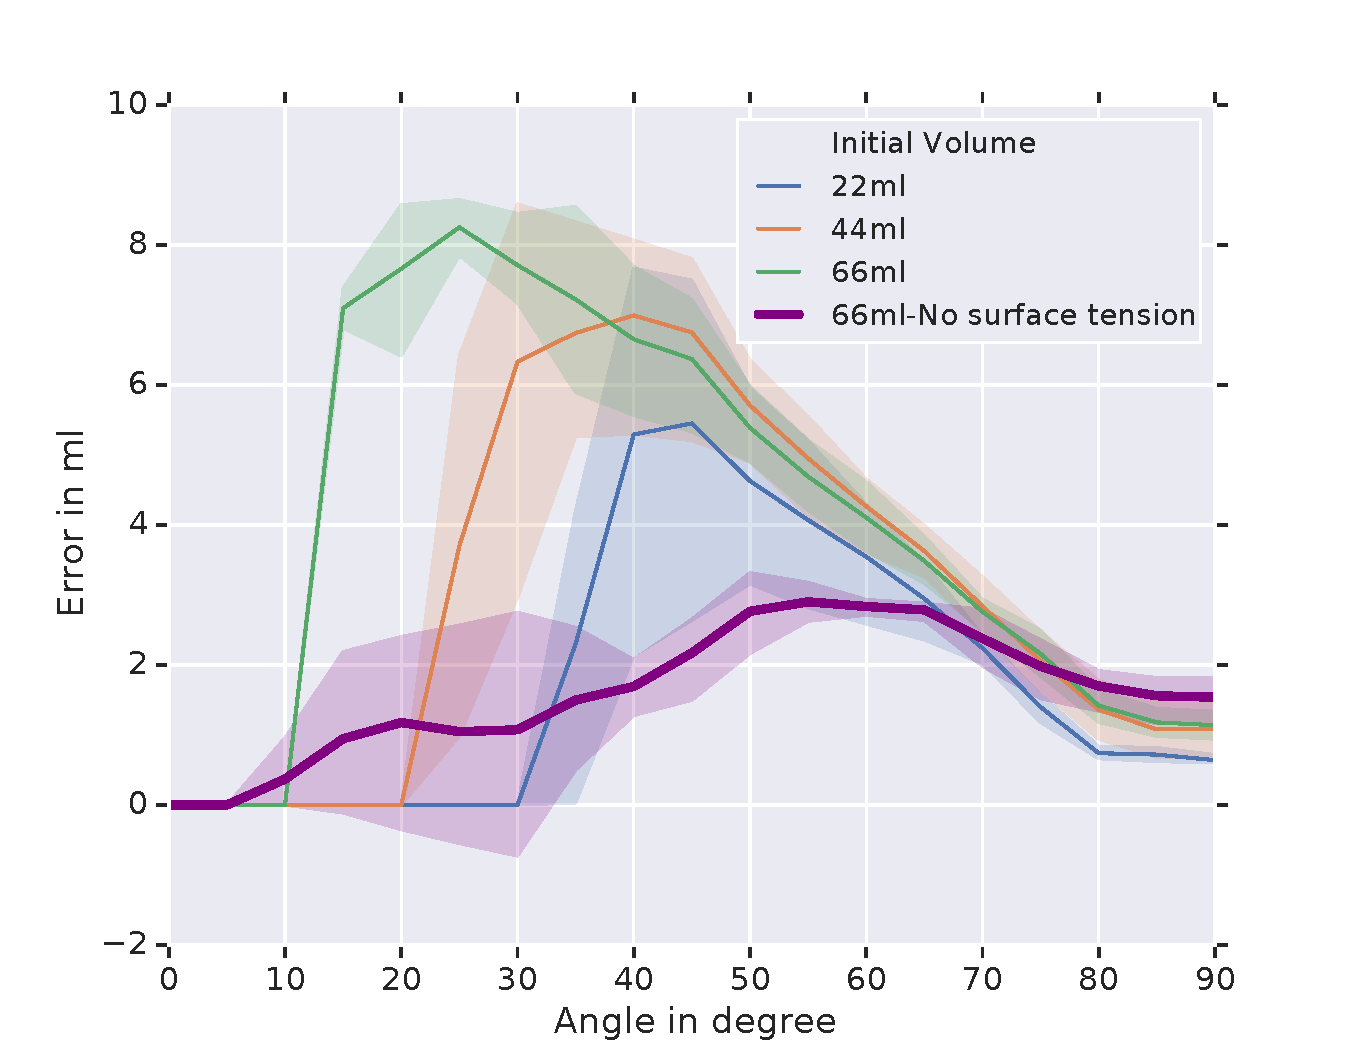
\includegraphics[width=1\textwidth]{fig/chp_pouring/Method2-ST-Cup3-Error.pdf}
		\caption{Errors with Cup~3}
		\label{fig:pour_method-exp1.sub2}
	\end{subfigure}
	\caption{Influence of Surface Tension on Method 2. In Figure \ref{fig:pour_method-exp1.sub1}, the blue, orange, and greeb lines show the results of Cup~2 with initial volumes of 30, 60, and 90\,ml, respectively. Cup~3 is 22, 44, and 66\,ml (Figure \ref{fig:pour_method-exp1.sub2}). The purple line shows the result with no surface tension and Cup~2 with an initial volume of 90\,ml.}
	\label{fig:pour_method-exp1}
\end{figure*}
% ------------------------------------------------------------------------------------

結果は図\ref{fig:pour_method-exp1}にしめした．
表面張力ありの条件では，注ぎ開始直後に $-10\,\mathrm{ml}$ から
$-5\,\mathrm{ml}$ の範囲に誤差が集中し，注ぎの進行とともに
誤差が減少する傾向が確認された．
一方，表面張力なし条件では，誤差の平均は 1.57\,ml，
標準偏差は 0.93\,ml まで大幅に低減した．

\textbf{考察：}
表面張力の有無による比較実験から，表面張力が注いだ体積積推定に与える影響が定量的に明らかとなった．
表面張力ありの条件では，注ぎ開始直後に$-10$\,mlから$-5$\,mlの範囲に誤差が集中し，
注ぎの進行とともに誤差が減少する傾向が認められた．
これは，注ぎ縁付近において液体と容器壁面の間に働く表面張力により液面が約3\,mm盛り上がるために，
実際に注がれた体積が推測値より小さくなることに起因する．
注ぎが進むにつれて液体と容器縁の接触面積が減少し，表面張力も徐々に弱まるため，誤差が収束する．
一方，容器の縁に洗剤を薄く塗布して表面張力を弱めた条件では，
容器2の最大誤差は約3\,ml，容器3の最大誤差は約7\,mlまで低減した．
ただし容器3では注ぎ開始直後に大量の水とともに洗剤が流れ出るため，
初期角度以降は表面張力低減効果が失われ，若干の誤差が残留した．
両条件の差から，表面張力の影響は容器3で最大約10\,ml程度と推定され，
容器2では約5\,mlとより小さいことが分かった．
これらの結果は，手法2において表面張力を考慮した補償の重要性を示している．


\subsubsection{手法2注ぎ精度の検証}
\label{sec:pour_exp_method2_all}

\textbf{実験方法：}  
表面張力の影響を含めた上で，手法2の総合的な注ぎ精度を評価した．  
実験には容器2および容器3を用いた．  
容器2では初期液体体積を100\,mlに，容器3では70\,mlに固定し，  
目標体積をそれぞれ0--95\,ml，0--65\,mlの範囲で5\,ml刻みに設定した．  
各目標体積につき4回の注ぎ試行を実施し，毎回新たに容器モデルを取得した．  
注ぎ動作は，\ref{sec:pour_angle_volume}節で求めた傾き角度と注いだ体積の関係に基づき，  
目標体積に対応する目標角度までP制御により容器を回転させる方法で行った．  
目標角度に到達後は残留液体の流出を待機し，戻し動作を実行した．

\textbf{実験結果：}  

% -------------------- IROS2019 Fig. Method2-ExpAll-Error --------------------
\begin{figure}[t]
	\centering
	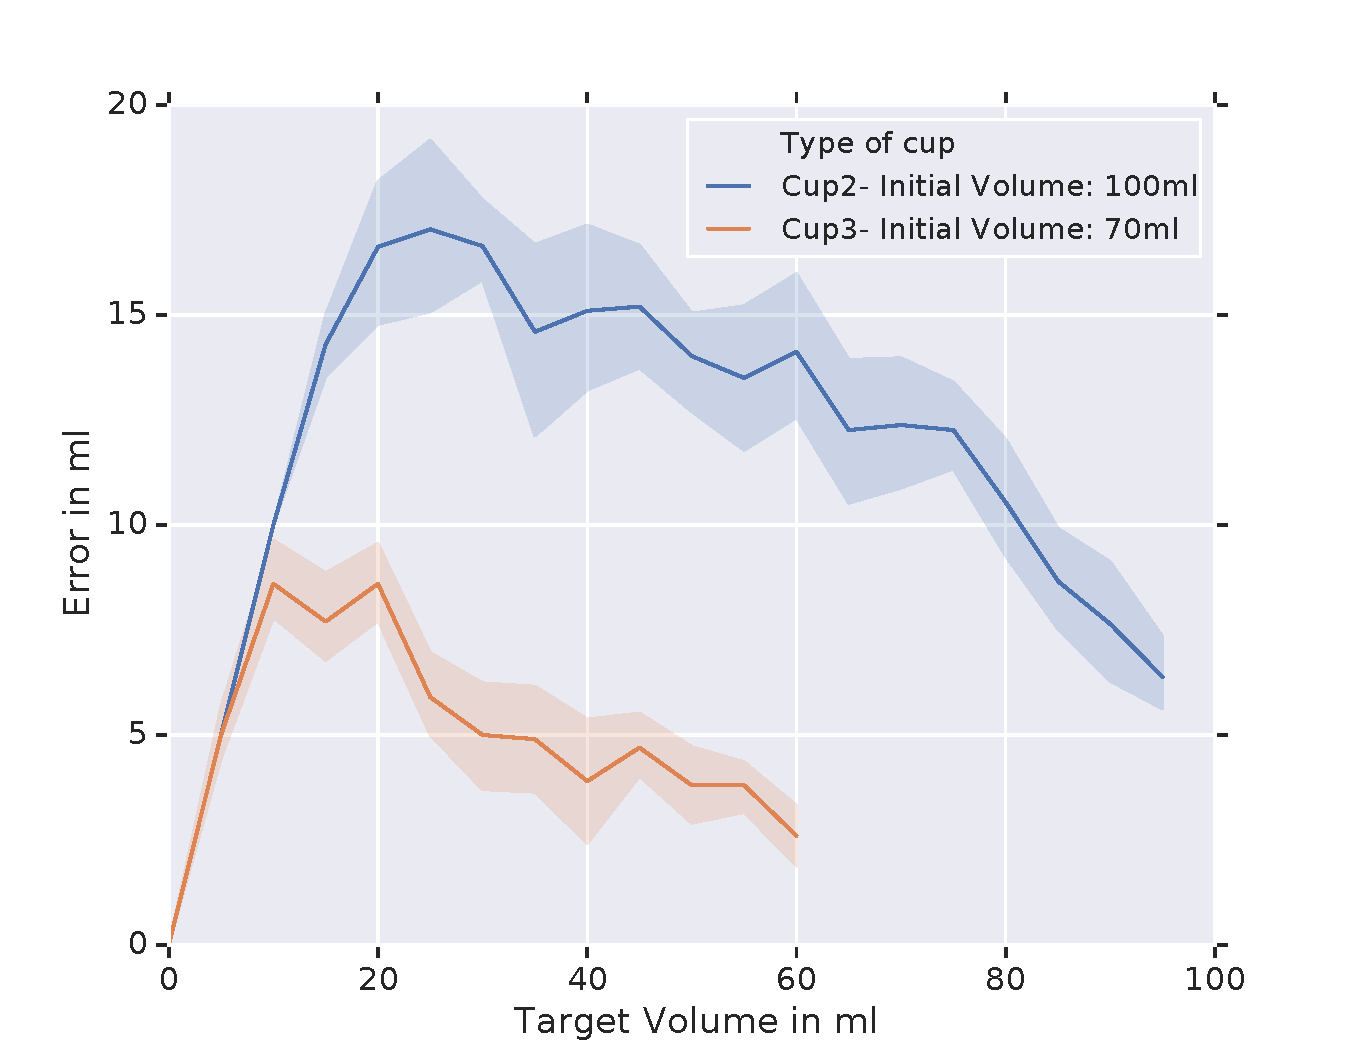
\includegraphics[width=0.9\linewidth]{fig/chp_pouring/Method2-ExpAll-Error.pdf}
	\caption{Errors of Method 2}
	\label{fig:pour_Method2-Cup2-Error}
\end{figure}
% ---------------------------------------------------------------------------

表\ref{tab:pour_method2_error}に誤差の平均と標準偏差を示す．

\begin{table}[h]
	\caption{The average (Avg.) and standard deviation (S.d.) of errors in  Method~2}
	\label{tab:pour_method2_error}
	\centering
	\begin{tabular}{ccc}
		\toprule 
		& Cup 2 & Cup 3 \\ 
		\midrule
		Avg. (ml)		& 11.88  & 4.96  \\ 
		S.D. (ml)		& 4.63  & 2.57 \\ 
		\bottomrule
	\end{tabular}
\end{table}
\textbf{考察：}
手法2の総合的な注ぎ精度は，容器2で平均誤差11.88\,ml，標準偏差4.63\,ml，
容器3で平均誤差4.96\,ml，標準偏差2.57\,mlとなり，手法1に比べて精度が劣ることが明らかとなった．
主な誤差要因は，注ぐ容器の内部点群が取得できないために外側点群からモデルを構築することによる
壁の厚さの影響と，表面張力の影響である．
容器2の最大誤差は約18\,mlに達しており，これは表面張力影響実験の結果と整合する．
また容器3では，表面張力の影響が最大約10\,mlと推定されることに加え，外側点群を用いることで
容器底部の厚さが容積計算に誤差をもたらしている．
手法2は注ぎ実行中の液面監視を必要とせず，カメラ配置の自由度が低い環境でも動作可能という
利点があるが，高精度が要求される場面では手法1の方が適していることが示された．

\subsection{両手法の比較考察}
\label{sec:pour_exp_discussion}

両手法の実験結果をまとめ，以下の比較考察が得られる．

% \begin{table}[t]
%   \centering
%   \caption{手法1 と 手法2 の比較}
%   \label{tab:pour_method_comparison}
%   \begin{tabular}{@{}p{0.28\textwidth}p{0.31\textwidth}p{0.31\textwidth}@{}}
%     \toprule
%     比較項目 & 手法1（注ぎ先容器基準） & 手法2（注ぐ容器基準） \\
%     \midrule
%     制御方式 & PD制御（注いだ体積積フィードバック） & P制御（角度追跡） \\
%     \midrule
%     精度（容器3） & 平均$-0.95\,\mathrm{ml}$ & 平均$4.96\,\mathrm{ml}$ \\
%     \midrule
%     主な誤差要因 & 液面検出精度 & 表面張力，容器壁の厚さ・変形 \\
%     \midrule
%     必要情報 & 注ぎ先容器内部形状 & 注ぐ容器形状＋初期液体体積 \\
%     \midrule
%     利点 & 高精度，注ぐ容器が未知でも可 &
%     注ぎ先容器の内部観測不要，実行中の液面監視不要 \\
%     \midrule
%     欠点 & 注いでいる間の液面観測必須 &
%     表面張力の影響が大きい，容器の個体差（壁の厚さ・変形）に敏感 \\
%     \bottomrule
%   \end{tabular}
% \end{table}

% TODO: 表格出去了。。。
\begin{table}[!t]
  \centering
  \caption{Comparison of Method 1 and Method 2}
  \label{tab:pour_method_comparison}
    \begingroup
  \footnotesize
  \setlength{\tabcolsep}{4pt}
  \renewcommand{\arraystretch}{0.95}
  \begin{tabularx}{.75\textwidth}{@{}p{0.28\textwidth}p{0.31\textwidth}p{0.31\textwidth}@{}}
    \toprule
    Item & Method 1 (target container based) & Method 2 (pouring container based) \\
    \midrule
    Control method & PD control (poured volume feedback) & P control (angle tracking) \\
    \midrule
    Accuracy (Cup 3) & Mean $-0.95\,\mathrm{ml}$ & Mean $4.96\,\mathrm{ml}$ \\
    \midrule
    Main error sources & Liquid level detection accuracy & Surface tension, container wall thickness \& deformation \\
    \midrule
    Required information & Internal shape of target container & Shape of pouring container and initial liquid volume \\
    \midrule
    Advantages & High accuracy; pouring container can be unknown &
    No need to observe interior of target container; no real-time liquid level monitoring required \\
    \midrule
    Disadvantages & Requires liquid level observation during pouring &
    Largely affected by surface tension; sensitive to container individual differences (wall thickness, deformation) \\
    \bottomrule
  \end{tabularx}
  \endgroup
\end{table}

\begin{enumerate}
  \item \textbf{精度：}  
  手法1（容器3における平均誤差 $-0.95\,\mathrm{ml}$，標準偏差 $1.16\,\mathrm{ml}$）は，手法2（同容器で平均誤差 $4.96\,\mathrm{ml}$，標準偏差 $2.57\,\mathrm{ml}$）より高い精度を達成した．  
  \revise{手法1の容器3での誤差は，事前学習や事前モデルを前提とする先行研究（約 $38\,\mathrm{ml}$ の誤差\cite{Related1}，約 $5\,\mathrm{ml}$ の誤差\cite{Related2}）と比較して小さい．ただし，容器1では平均誤差が7.35\,mlであり，精度は容器形状と観測条件に依存する．}
  \item \textbf{実装要件：}  
  手法1は注ぎ中の液面をリアルタイムに観測する必要があり，カメラ視野の確保や液面と容器縁の連結時への対策が不可欠である．  
  一方，手法2は事前の幾何計算のみで制御が完結するため，実装の制約が少ない．  
  \item \textbf{誤差要因の性質：}  
  手法1の誤差は主に液面検出精度（容器形状や液体の光学的性質に依存）に起因する．  
  手法2の誤差は主に表面張力および容器の壁の厚さ・変形（容器の物理的特性）に起因し，容器の個体差の影響を受けやすい．  
  \item \textbf{両手法の使い分け：}  
  \revise{高い定量性が要求される場合には，内面と液面を安定に観測できるなら手法1を優先する．一方，カメラ配置の自由度が低い環境や，大量の液体を注ぐため表面張力の相対的な影響が小さい場合には，手法2を選択できる．少量の調味料については，本実験の誤差を許容できるかをレシピ側の要求量と比較し，必要なら計量スプーンや秤を用いる．}
\end{enumerate}

\begin{revisionblock}
\subsection{家庭内の注ぎ作業としての評価}
家庭料理では小さじ1杯が約5\,mlであることを実用上の目安とすると，手法1の容器3では平均誤差の絶対値が1\,ml未満であり，観測しやすい容器へ比較的少量を注ぐ用途に可能性がある．
一方，手法1の容器1では平均7.35\,ml，手法2では容器2で11.88\,ml，容器3で4.96\,mlの誤差があり，小量の調味料では味への影響を無視できない．
手法2は液面を実時間観測しない利点があるため，水やだしなど比較的大きな量を移す用途に適するが，表面張力，容器壁厚，初期量の誤差を含む．

本実験で秤を用いたのは注いだ体積の真値を得る評価のためであり，提案制御への入力には用いていない．
したがって，「外部計測道具を用いない」とは制御時に補助計量器を用いないことを意味する．
現状は不透明な低粘性液体と三種類の開口容器に限られ，透明液体，粘性液体，泡，こぼれ，衛生・清掃，容器の再把持を含む家庭の一連作業は評価していない．
本章が示したのは，これらの条件下で，容器形状を直接利用して指定量に対応する制御目標を作れることである．
\end{revisionblock}


% ============================================================================
\section{本章のまとめ}
\label{sec:pour_summary}
% ============================================================================

\revise{本章では，事前登録していない容器の3D点群と，手法ごとに必要な液面または初期液体量を入力とし，注いだ体積または目標傾斜角度を出力して，指定量を注ぐ二つのタスク固有手法を示した．}
手法1は注ぎ先容器の液面高さを体積へ変換し，体積誤差に基づくPD制御を行う．
手法2は注ぐ容器の注ぎ縁と注ぐポイントを検出し，容器角度と注いだ体積の関係から目標角度を求めてP制御を行う．

これらの手法を実現した本章の成果は，以下の三点にまとめられる．
\begin{enumerate}
  \item \textbf{幾何学的な分析手法の応用：} 
    容器の3D点群モデルを基盤とし，
    (a) RANSACに基づくリアルタイム液面検出と注いだ体積への変換，
    (b) ConvexHullと複数姿勢投票による注ぎ縁・注ぐポイントの安定な検出，
    (c) 注ぎ角度--注いだ体積関係の計算
    の一連の幾何学的な分析手法を提案した．
  \item \textbf{分析結果に基づく動作制御の実装：}
    幾何学的な分析の結果を動作制御へ接続するため，
    手法1（注いだ体積フィードバックPD制御＋戻し動作）と
    手法2（目標角度追跡P制御＋残留液流出待機＋戻し動作）
    の2つの制御手法を設計・実装した．
  \item \textbf{実機実験による検証：}
    形状特性の異なる3種類の容器を用いた総計80回以上の注ぎ実験を通じて，
    手法1 では最小平均誤差 $-0.95\,\mathrm{ml}$（容器3），
    手法2 では平均誤差 $4.96\,\mathrm{ml}$（容器3）の精度を達成した．
    \revise{これにより，制御時に外部計量器を用いず，三種類の容器と設定した液体条件の範囲で定量注ぎが可能であることを示した．最小誤差は手法1・容器3の$-0.95\pm1.16$\,mlであったが，手法1・容器1では$7.35\pm5.45$\,ml，手法2・容器2では$11.88\pm4.63$\,mlであり，家庭用途への適否は容器，観測条件，およびレシピが許容する誤差に依存する．}
\end{enumerate}

本章の結果は，第\ref{ch:introduction}章\ref{tab:tasks}表に示した
検証作業のうち，「容器という環境を利用した流体操作」に対応するものであり，
\revise{容器という環境の幾何を液量または角度へ変換することで，直接把持できない液体に対する操作量を決定できることを示した．ただし，容器形状に依存する誤差，表面張力，粘性，観測困難な液面への対応は適用範囲外または今後の課題である．}
次章では，形状と環境の分析を中心とした本章から，包丁外力に抵抗する把持安定性の分析へ進む．食材形状，包丁軌道を同時に用い，力学的・環境的な分析から把持位置を決定する．

% 今後の課題として，ConcaveHull を用いた断面処理による凹型容器への拡張，
% 表面張力を考慮した角度--注いだ体積関係の補償モデルの導入，
% および液体の粘性が高い場合への対応が挙げられる．
